% Created by tikzDevice version 0.12.6 on 2026-05-14 20:42:29
% !TEX encoding = UTF-8 Unicode
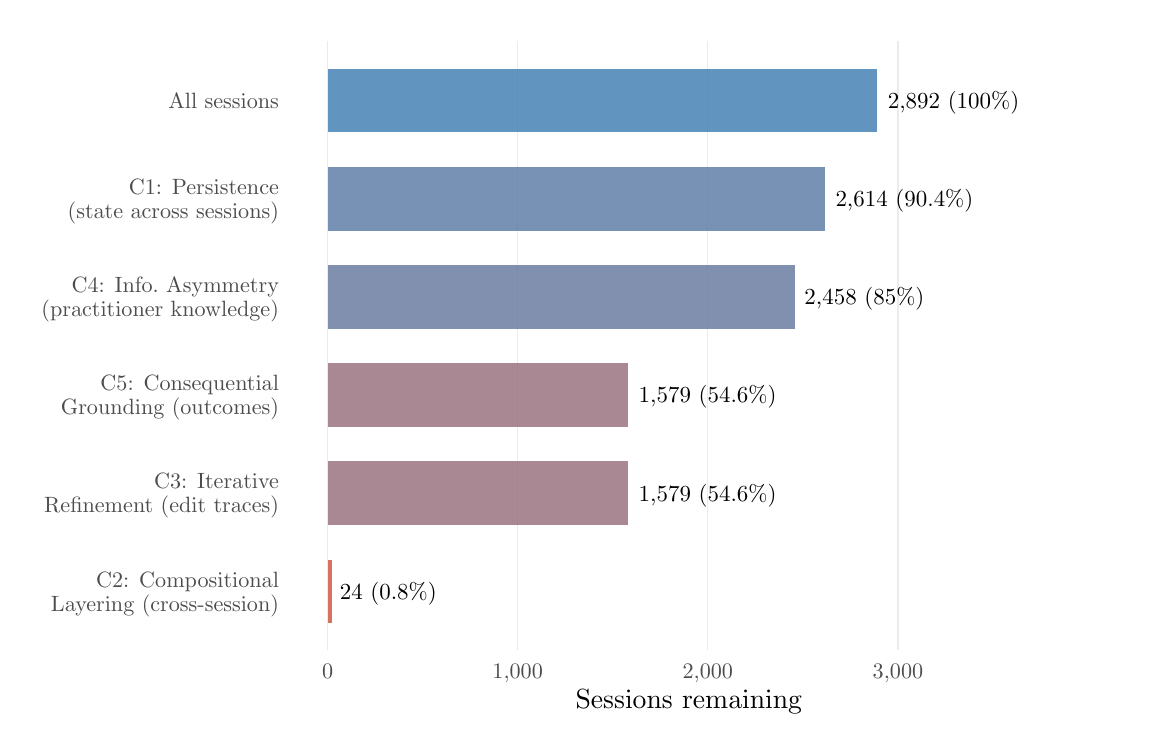
\begin{tikzpicture}[x=1pt,y=1pt]
\definecolor{fillColor}{RGB}{255,255,255}
\path[use as bounding box,fill=fillColor,fill opacity=0.00] (0,0) rectangle (397.48,252.94);
\begin{scope}
\path[clip] (  0.00,  0.00) rectangle (397.48,252.94);
\definecolor{fillColor}{RGB}{255,255,255}

\path[fill=fillColor] (  0.00,  0.00) rectangle (397.48,252.94);
\end{scope}
\begin{scope}
\path[clip] ( 95.30, 27.90) rectangle (382.48,247.95);
\definecolor{drawColor}{gray}{0.92}

\path[draw=drawColor,line width= 0.5pt,line join=round] (108.36, 27.90) --
	(108.36,247.95);

\path[draw=drawColor,line width= 0.5pt,line join=round] (177.06, 27.90) --
	(177.06,247.95);

\path[draw=drawColor,line width= 0.5pt,line join=round] (245.76, 27.90) --
	(245.76,247.95);

\path[draw=drawColor,line width= 0.5pt,line join=round] (314.47, 27.90) --
	(314.47,247.95);
\definecolor{fillColor}{RGB}{70,130,180}

\path[fill=fillColor,fill opacity=0.85] (108.36,215.12) rectangle (307.05,238.18);
\definecolor{fillColor}{RGB}{97,127,169}

\path[fill=fillColor,fill opacity=0.85] (108.36,179.62) rectangle (287.95,202.69);
\definecolor{fillColor}{RGB}{109,125,163}

\path[fill=fillColor,fill opacity=0.85] (108.36,144.13) rectangle (277.23,167.20);
\definecolor{fillColor}{RGB}{154,115,129}

\path[fill=fillColor,fill opacity=0.85] (108.36,108.64) rectangle (216.84,131.71);

\path[fill=fillColor,fill opacity=0.85] (108.36, 73.15) rectangle (216.84, 96.22);
\definecolor{fillColor}{RGB}{205,91,69}

\path[fill=fillColor,fill opacity=0.85] (108.36, 37.66) rectangle (110.00, 60.73);
\definecolor{drawColor}{RGB}{0,0,0}

\node[text=drawColor,anchor=base west,inner sep=0pt, outer sep=0pt, scale=  0.83] at (310.82,223.81) {2{,}892 (100\%)};

\node[text=drawColor,anchor=base west,inner sep=0pt, outer sep=0pt, scale=  0.83] at (291.91,188.32) {2{,}614 (90.4\%)};

\node[text=drawColor,anchor=base west,inner sep=0pt, outer sep=0pt, scale=  0.83] at (280.68,152.83) {2{,}458 (85\%)};

\node[text=drawColor,anchor=base west,inner sep=0pt, outer sep=0pt, scale=  0.83] at (220.80,117.33) {1{,}579 (54.6\%)};

\node[text=drawColor,anchor=base west,inner sep=0pt, outer sep=0pt, scale=  0.83] at (220.80, 81.84) {1{,}579 (54.6\%)};

\node[text=drawColor,anchor=base west,inner sep=0pt, outer sep=0pt, scale=  0.83] at (112.79, 46.35) {     24 (0.8\%)};
\end{scope}
\begin{scope}
\path[clip] (  0.00,  0.00) rectangle (397.48,252.94);
\definecolor{drawColor}{gray}{0.30}

\node[text=drawColor,anchor=base east,inner sep=0pt, outer sep=0pt, scale=  0.80] at ( 90.80, 50.76) {C2: Compositional};

\node[text=drawColor,anchor=base east,inner sep=0pt, outer sep=0pt, scale=  0.80] at ( 90.80, 42.12) {Layering (cross-session)};

\node[text=drawColor,anchor=base east,inner sep=0pt, outer sep=0pt, scale=  0.80] at ( 90.80, 86.25) {C3: Iterative};

\node[text=drawColor,anchor=base east,inner sep=0pt, outer sep=0pt, scale=  0.80] at ( 90.80, 77.61) {Refinement (edit traces)};

\node[text=drawColor,anchor=base east,inner sep=0pt, outer sep=0pt, scale=  0.80] at ( 90.80,121.74) {C5: Consequential};

\node[text=drawColor,anchor=base east,inner sep=0pt, outer sep=0pt, scale=  0.80] at ( 90.80,113.10) {Grounding (outcomes)};

\node[text=drawColor,anchor=base east,inner sep=0pt, outer sep=0pt, scale=  0.80] at ( 90.80,157.23) {C4: Info.\ Asymmetry};

\node[text=drawColor,anchor=base east,inner sep=0pt, outer sep=0pt, scale=  0.80] at ( 90.80,148.59) {(practitioner knowledge)};

\node[text=drawColor,anchor=base east,inner sep=0pt, outer sep=0pt, scale=  0.80] at ( 90.80,192.72) {C1: Persistence};

\node[text=drawColor,anchor=base east,inner sep=0pt, outer sep=0pt, scale=  0.80] at ( 90.80,184.08) {(state across sessions)};

\node[text=drawColor,anchor=base east,inner sep=0pt, outer sep=0pt, scale=  0.80] at ( 90.80,223.90) {All sessions};
\end{scope}
\begin{scope}
\path[clip] (  0.00,  0.00) rectangle (397.48,252.94);
\definecolor{drawColor}{gray}{0.30}

\node[text=drawColor,anchor=base,inner sep=0pt, outer sep=0pt, scale=  0.80] at (108.36, 17.89) {    0};

\node[text=drawColor,anchor=base,inner sep=0pt, outer sep=0pt, scale=  0.80] at (177.06, 17.89) {1,000};

\node[text=drawColor,anchor=base,inner sep=0pt, outer sep=0pt, scale=  0.80] at (245.76, 17.89) {2,000};

\node[text=drawColor,anchor=base,inner sep=0pt, outer sep=0pt, scale=  0.80] at (314.47, 17.89) {3,000};
\end{scope}
\begin{scope}
\path[clip] (  0.00,  0.00) rectangle (397.48,252.94);
\definecolor{drawColor}{RGB}{0,0,0}

\node[text=drawColor,anchor=base,inner sep=0pt, outer sep=0pt, scale=  1.00] at (238.89,  6.94) {Sessions remaining};
\end{scope}
\end{tikzpicture}
